\documentclass[14pt]{beamer} 
\usetheme{default}

\usepackage{import}
\usepackage{graphicx}
\usepackage{amsmath}
\usepackage{amssymb}
\usepackage{amsthm}

\usepackage{tikz}
\usetikzlibrary{arrows}
\usetikzlibrary{shapes, arrows.meta}

\usepackage[absolute, overlay]{textpos}

\usepackage{pgfplots}
\usepackage[T1]{fontenc}
\usepackage{lmodern}
\usepackage[utf8]{inputenc}

\usepackage{caption}
\usepackage{subcaption}
\usepackage{../tex/mathpartir}

%\setbeamercovered{transparent}
\definecolor{bgcol}{rgb}{0.8, 0.8, 0.8}
\setbeamercolor{bgcolor}{fg=black,bg=bgcol}

\definecolor{green}{rgb}{0.0, 0.5, 0.0}
\definecolor{red}{rgb}{0.8, 0.0, 0.0}

\newcommand{\Type}{\mathsf{Type}}
\newcommand{\Space}{\mathsf{Space}}
\newcommand{\Open}{\mathsf{Open}}
\newcommand{\PLower}{\mathcal{P}}
\newcommand{\PUpper}{\mathcal{P}_\square}
\newcommand{\Prob}{\mathcal{R}}
\newcommand{\State}{\mathsf{State}}

\newcommand{\cov}{\vartriangleleft}
\newcommand{\nat}{\mathbb{N}}
\newcommand{\suchthat}{\ |\ }
\newcommand{\List}[1]{\mathsf{list}\ {#1}}
\newcommand{\rat}{\mathbb{Q}}
\newcommand{\R}{\mathbb{R}}
\newcommand{\bool}{\texttt{bool}}
\newcommand{\Prop}{\mathbb{P}}
\newcommand{\Dist}[1]{\mathcal{P}({#1})}
\newcommand{\fun}[2]{\lambda\ {#1}\Rightarrow{#2}}
\newcommand{\ret}[1]{\mathsf{ret}_{#1}}

\newcommand*\circled[1]{\tikz[baseline=(char.base)]{
            \node[shape=circle,draw,inner sep=2pt,thick] (char) {#1};}}
            
\newcommand{\dirsup}{\mathop{\setlength{\unitlength}{.7em}\raisebox{-.2em}%
    {\begin{picture}(1,1.5)\put(.5,0){\line(-1,3){.48}}
    \put(.5,0){\vector(1,3){.5}}\end{picture}}}} 
            
\newcommand*{\tikzbullet}[2]{%
  \setbox0=\hbox{\strut}%
  \begin{tikzpicture}
    \useasboundingbox (-.25em,0) rectangle (.25em,\ht0);
    \filldraw[draw=#1,fill=#2] (0,0.3\ht0) circle[radius=.25em];
  \end{tikzpicture}%
}

\newcommand{\SafeToGo}{\tikzbullet{green}{green}}
\newcommand{\SafeToStop}{\tikzbullet{red}{red}}

\title{Programming with continuous spaces}
\author{\textbf{Ben Sherman}, Luke Sciarappa, Michael Carbin, Adam Chlipala}
\date{November 6, 2016}

\setbeamertemplate{footline}{%
  \raisebox{5pt}{\makebox[\paperwidth]{\hfill\makebox[10pt]{\scriptsize\insertframenumber}}}}
\setbeamertemplate{navigation symbols}{}
%\setbeamertemplate{headline}
%{\vspace{0.03em}
%\begin{beamercolorbox}[wd=\paperwidth,ht=4ex,dp=1ex,center]{bgcolor}
% \small \insertshorttitle
%  \end{beamercolorbox}
%}
\begin{document}

\maketitle

\begin{frame}
\begin{center}
\includegraphics[width=0.6\textwidth]{../2016-NEPLS/images/autonomous-car.jpg}
\\
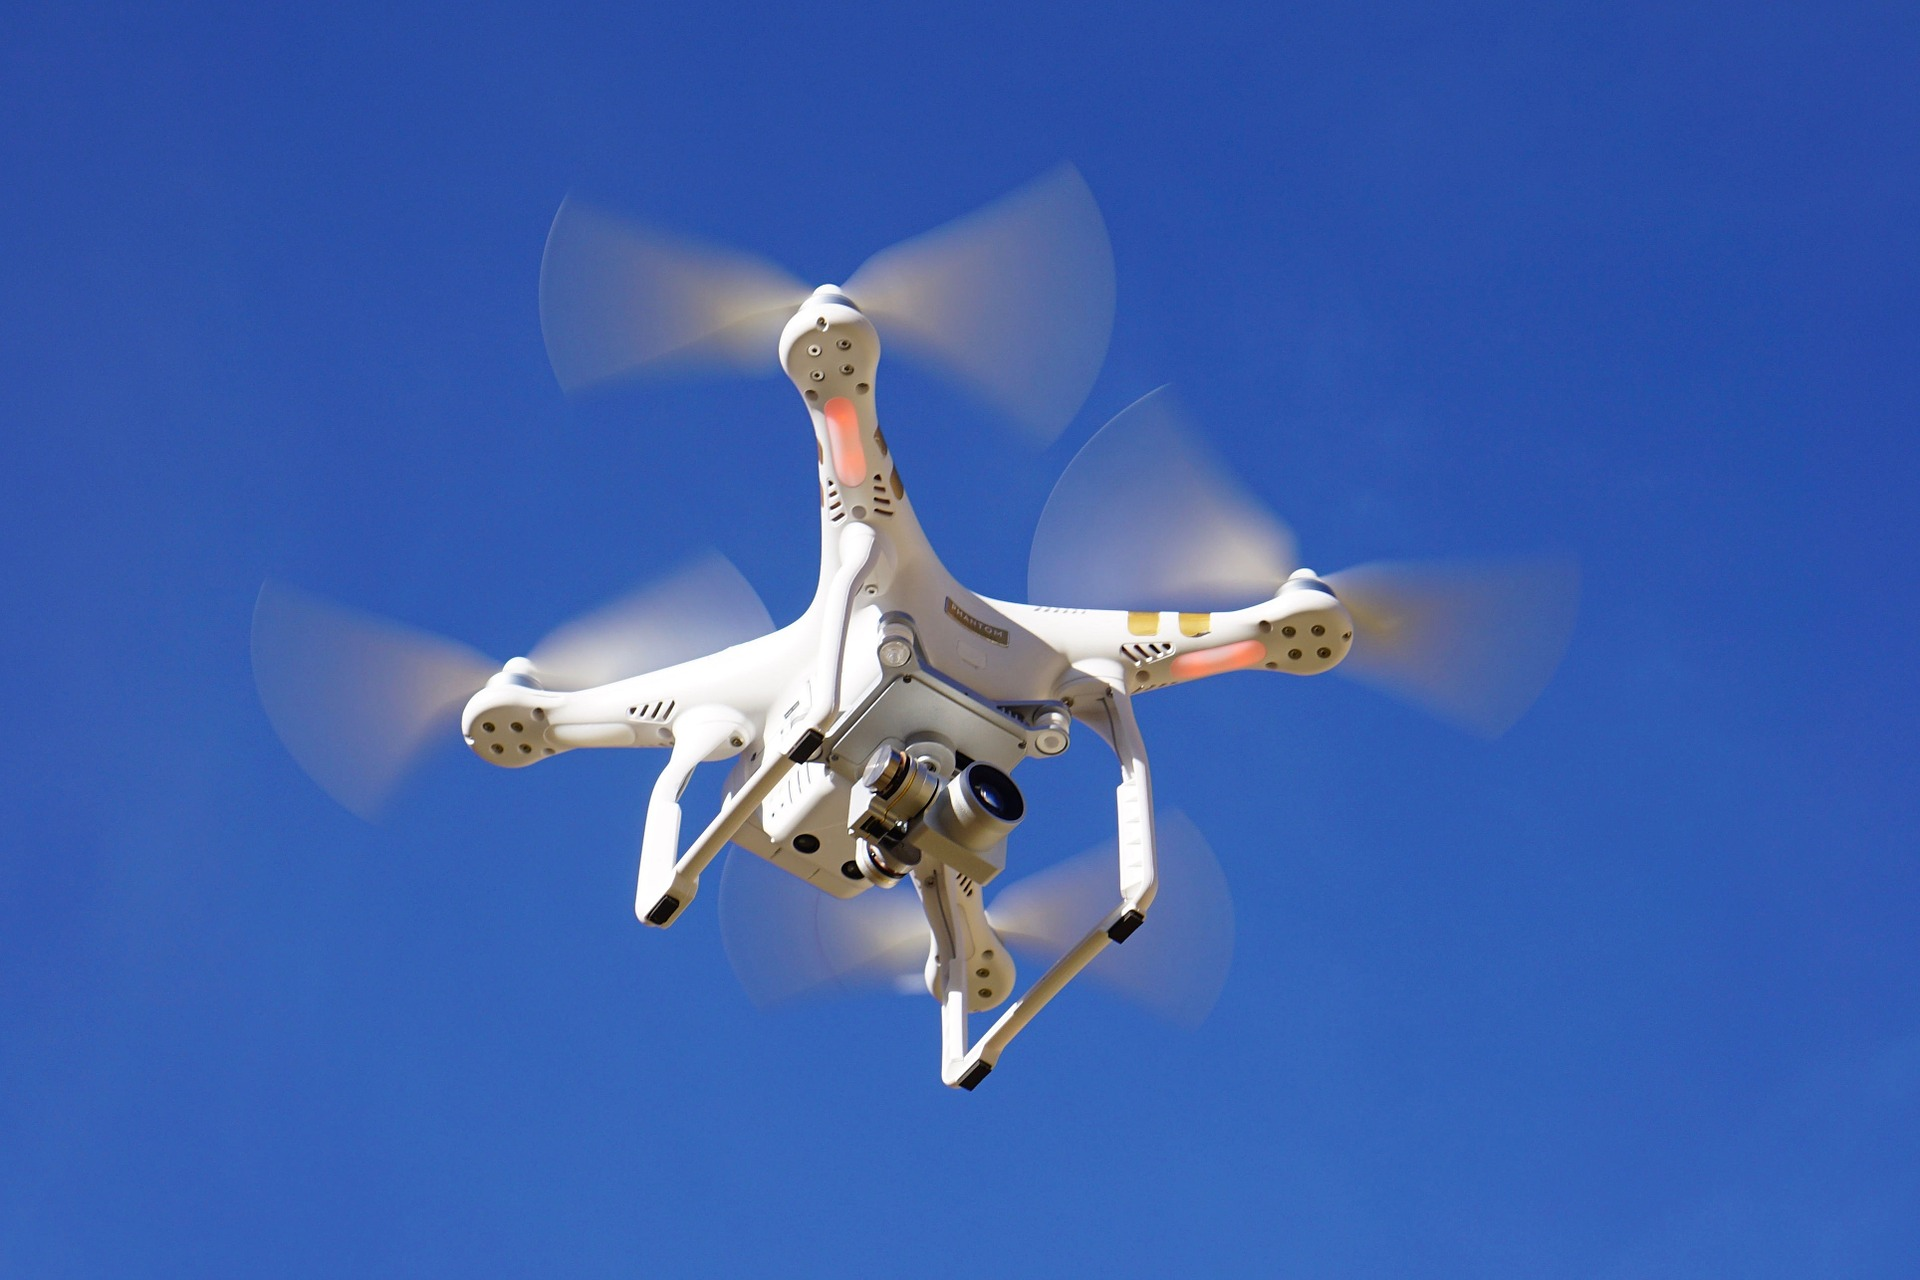
\includegraphics[width=0.6\textwidth]{../2016-NEPLS/images/drone.jpg}
\end{center}
\end{frame}

\note{
\small
Software is increasingly applied to safety-critical domains which involve computing with continuous values, such as space, time, probability, and quantity. Cyber-physical systems such as autonomous cars, drones, and rockets must interact with the continuous world, and software errors can be catastrophic.

In domains where software correctness is paramount, construction of formal proofs has been successful. But there are many additional complications for software dealing with continuous values. Definitions of correctness are not so straightforward, and often requiring reasoning about either probabilistic or worst-case uncertainty. Additionally, computations used, such as floating point, aren't mathematically sound.
}

\begin{frame}
\begin{center}
\huge Challenge: gap between the \textbf{code} and the \textbf{math}
\end{center}

\bigskip
\pause 
\begin{itemize}
  \item Overflow, rounding errors
  \item Mathematical identities fail
  \item Probabilistic semantics are difficult/unclear
  \item Proofs about continuous models invalid
\end{itemize}
\end{frame}

\begin{frame}
\begin{center}
\huge Program literally with continuous spaces!
\end{center}
\end{frame}

\begin{frame}{PL for continuous spaces}

\begin{center}
\Large
\begin{align*}
\text{types} &\triangleq \text{spaces}
\\
\text{values} &\triangleq \text{points}
\\
\text{functions} &\triangleq \text{continuous maps}
\end{align*}
\end{center}
\end{frame}

\begin{frame}{Running points}
\begin{center}
\only<1>{\resizebox{0.7\textwidth}{!}{\import{../Figures/Cover/output/}{step1.pdf_tex}}}
\only<2>{\resizebox{0.7\textwidth}{!}{\import{../Figures/Cover/output/}{step2.pdf_tex}}}
\only<3>{\resizebox{0.7\textwidth}{!}{\import{../Figures/Cover/output/}{step3.pdf_tex}}}
\end{center}
\end{frame}


\begin{frame}{Buridan's autonomous car}

\begin{center}
\alt<3>
  {\Huge $\R \to \PLower(\bool)$}
  {\Huge $\R \to \bool$}
\normalsize
 \begin{tikzpicture}
 \draw [<->, ultra thick] (-5, 0) -- (5, 0);
  \node[below] (dec) at (0,-0.2) {0};
  \draw [ultra thick] (dec) --(0, 0.2);
 \draw [(->, ultra thick, green] (-2, 0.2) -- (5, 0.2);
 \draw [<-), ultra thick, red] (-5, 0.4) -- (2, 0.4);
 \node[inner sep=0pt, anchor=south] (car) at (-2.5, 0.6)
    {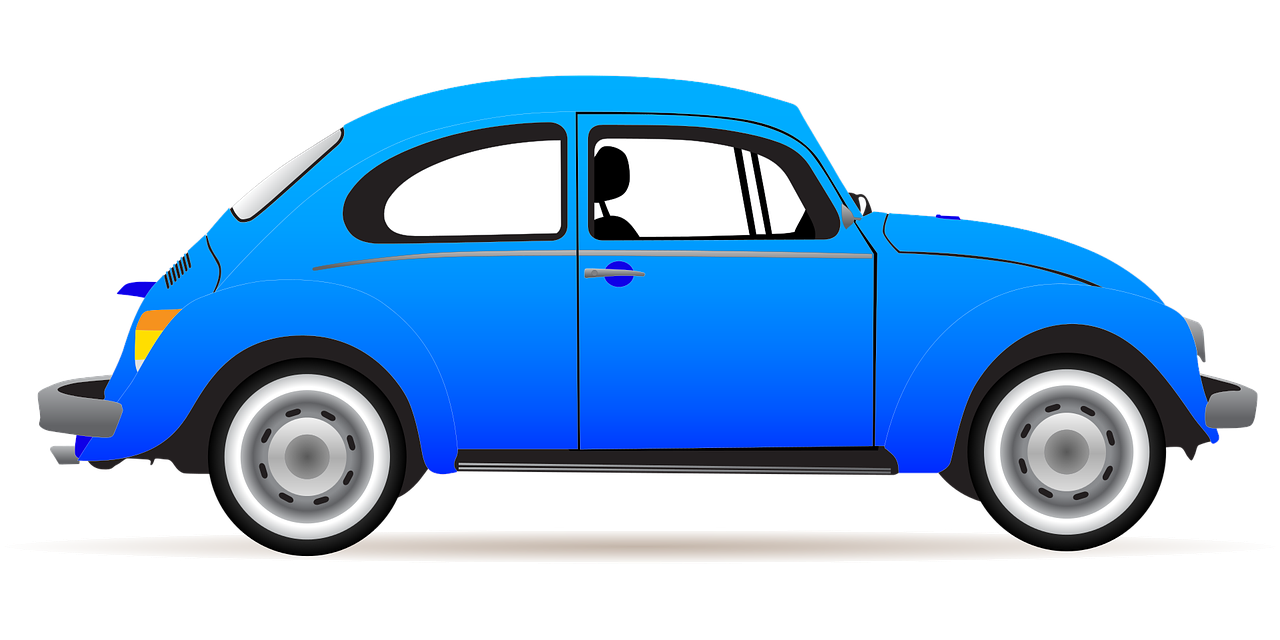
\includegraphics[width=.25\textwidth]{../2016-NEPLS/images/car.png}};
 \node[inner sep=0pt, anchor=south] (light) at (3.5,0.6)
    {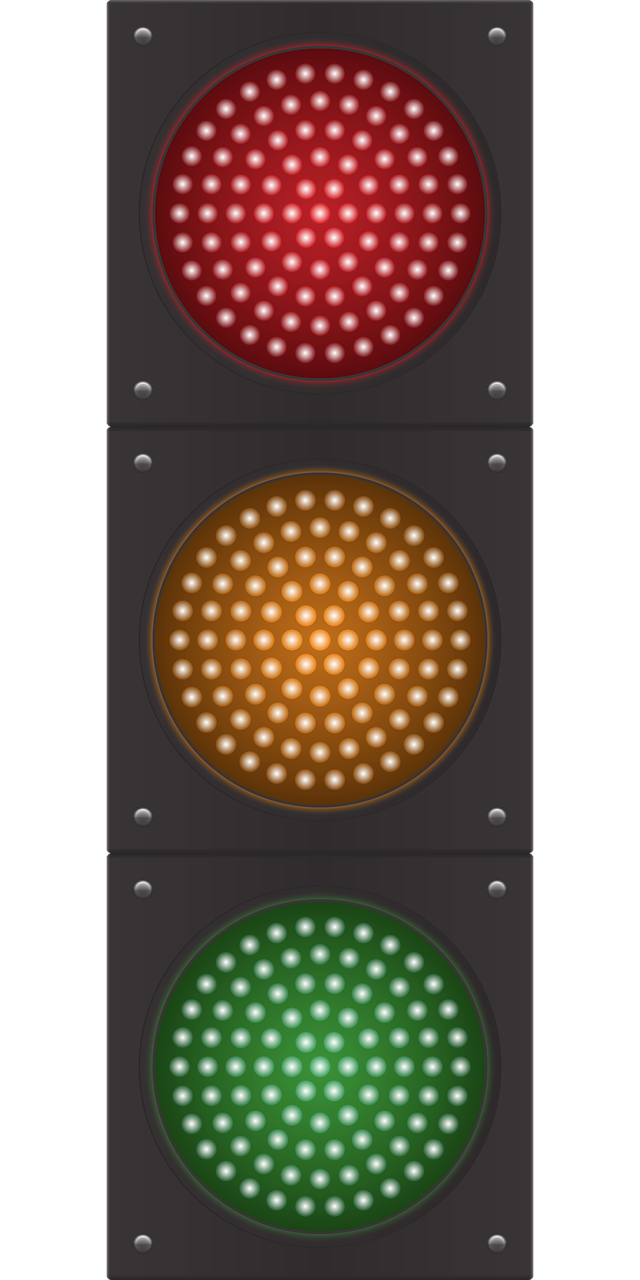
\includegraphics[width=.1\textwidth]{../2016-NEPLS/images/traffic-light.png}};
 \end{tikzpicture}
 \end{center}
\alt<3>{
\begin{align*}
\mathsf{brake?} &: \R \to \PLower(\bool)
\\ \mathsf{brake?}(x) &\triangleq \mathsf{cases}(x)
\begin{cases}
\SafeToGo
  \quad &\Longrightarrow \quad
  \{ \mathsf{false} \}
\\
\SafeToStop
  \quad &\Longrightarrow \quad
  \{ \mathsf{true} \}
\end{cases}
\end{align*}
 }
 {\invisible<1>{
 \begin{align*}
 \mathsf{brake?} &: \R \to \bool
\\ \mathsf{brake?}(x) &\triangleq x \le 0
 \end{align*}
 } }
 
\end{frame}

\end{document}

